% based on a template made by the university of cologne
% http://www.mi.uni-koeln.de/wp-MIEDV/wp-content/uploads/2016/07/LaTeX-Vorlage.zip - 2023-11-02
\documentclass[12pt,a4paper]{scrartcl}

\addtokomafont{sectioning}{\rmfamily}
%\usepackage[ngerman]{babel}% deutsches Sprachpaket wird geladen
\usepackage[T1]{fontenc} % westeuropäische Codierung wird verlangt
\usepackage[utf8]{inputenc}% Umlaute werden erlaubt
\usepackage[usenames]{color} % Erlaubt die Benutzung der namen im Farbpaket und deren Änderung
\usepackage{amsmath} % Erweiterung für den Mathe-Satz
\usepackage{amssymb} % alle Zeichen aus msam und msmb werden dargestellt
\usepackage{graphicx} % Graphiken und Bilder können eingebunden werden
%\usepackage{multirow} % erlaubt in einer Spalte einer Tabelle die Felder in mehreren Zeilen zusammenzufassen
\usepackage{enumerate} % erlaubt Nummerierungen
\usepackage{url} % Dient zur Auszeichnung von URLs; setzt die Adresse in Schreibmaschinenschrift.
\usepackage[center]{caption}  % Bildunterschrift wird zentriert
%\usepackage{subfigure} % mehrere Bilder können in einer fugure-Umgebung verwendet werden
%\usepackage{longtable} % Diese Umgebung ist ähnlich definiert wie die tabular-Umgebung, erlaubt jedoch mehrseitige Tabellen.
%\usepackage{paralist} % Modifikation der bereits bestehenden Listenumgebungen
\usepackage{lmodern}% Für die Schrift
\usepackage[hidelinks]{hyperref} % Links und Verweise werden innerhalb von PDF Dokumenten erzeugt
%\usepackage{wrapfig} % Das Paket ermöglicht es von Schrift umflossene Bilder und Tabellen einzufügen.
\usepackage{latexsym} % LaTeX-Symbole werden geladen
\usepackage{tikz} % Erlaubt es mit tikz zu zeichnen
\usepackage{tabularx} % Erlaubt Tabellen
\usepackage{algorithm} % Erlaubt Pseudocode
\usepackage{color} % Farbpaket wird geladen
%\usepackage{stmaryrd} % St Mary Road Symbole werden geladen
\usepackage{physics}

\numberwithin{equation}{section} % Nummerierungen der Gleichungen, die durch equation erstellt werden, sind gebunden an die section
\newcommand{\HRule}{\rule{\linewidth}{0.7mm}}
\newcommand{\pu}[1]{\ensuremath{\mathrm{#1}}}

% disable commands
\renewcommand{\[}{} % math block start
\renewcommand{\]}{\noindent} % math block end
\newcommand{\tightlist}{} % created in enumerations

\hypersetup{
  pdftitle={B 2.8},
  pdfcreator={LaTeX via pandoc}}

\setcounter{secnumdepth}{6}
\setcounter{tocdepth}{6}

\begin{document}
\begin{titlepage}
	\pagestyle{empty}

	\begin{center}

	\textsc{\LARGE Universität zu Köln }\\ [0.4cm]
	\textsc{Mathematisch-Naturwissenschaftliche Fakultät} \\[1.5cm]

	\includegraphics[width=0.45\textwidth]{uni}\\[1.5cm]  % Uni-Logo wird geladen

	\textsc{\Large Praktikum~B}\\[2mm]
	\textsc{}\\[10mm]
	\HRule \\[0.4cm]

		{	\Huge \bfseries B 2.8}\\[0.4cm]
			{	\huge \bfseries Versetzungen in \(\mathrm{LiF}\)}\\[0.3cm]
	
	\HRule \\[3cm]

			\textsc{\Large Catherine Tran } \\[3pt]
		\textsc{\Large Carlo Kleefisch } \\[3pt]
		\textsc{\Large Oliver Filla } \\[3pt]
		
% 	\begin{center}
% 	\textsc{\Large Catherine~Tran } \\[3pt]
% 	\textsc{\Large Carlo~Kleefisch } \\[3pt]
% 	\textsc{\Large Oliver~Filla } \\[3pt]
% 	\end{center}
	\end{center}
\end{titlepage}

\newpage
\tableofcontents
\newpage

\hypertarget{b2.8---versetzungen-in-mathrmlif}{%
\section{\texorpdfstring{B2.8 - Versetzungen in
\(\mathrm{LiF}\)}{B2.8 - Versetzungen in \textbackslash mathrm\{LiF\}}}\label{b2.8---versetzungen-in-mathrmlif}}

\hypertarget{theoretische-grundlagen}{%
\section{Theoretische Grundlagen}\label{theoretische-grundlagen}}

\hypertarget{kuxfcrzester-burgers-vektor-in-mathrmlif}{%
\subsection{\texorpdfstring{kürzester Burgers-Vektor in
\(\mathrm{LiF}\)}{kürzester Burgers-Vektor in \textbackslash mathrm\{LiF\}}}\label{kuxfcrzester-burgers-vektor-in-mathrmlif}}

Der kürzeste Burgers-Vektor \(\vec{b}_\mathrm{min}\) in \(\mathrm{LiF}\)
ist der \([\frac{1}{2}\,0\,\frac{1}{2}]\) Vektor in der
\(\braket{1\,1\,0}\) Richtung. Seine Länge bestimmt sich wie folgt.
Hierbei ist \(a=0.402\,\mathrm{nm}\) die Gitterkonstante von
\(\mathrm{LiF}\). \([5]\)

\[
\begin{eqnarray}
    \left|\vec{b}_\mathrm{min}\right|
        &=& \frac{1}{2} \cdot \sqrt{a^2 + a^2} \\
        &=& \frac{1}{2} \sqrt{2} a \\
        &=& \frac{a}{\sqrt{2}}
\end{eqnarray}
\]

Die Energie einer Versetzung ist proportional zum Quadrat des
Burgers-Vektors. Ein Defekt mit einem längeren Burgers-Vektor benötigt
daher eine viel größeren Energie, was Versetzungen mit längeren
Burgers-Vektoren sehr viel unwahrscheinlicher macht.

Aufgrund der sich abwechselnden Lithium- und Fluoratome in den
Richtungen \(\braket{1\,0\,0}\) und \(\braket{1\,1\,1}\) sind die
Burgers-Vektoren in diesen Richtungen doppelt so lang, da sie immer
zwischen gleichen Atomen liegen. Der Burgers-Vektor in der
\(\braket{1\,0\,0}\)-Richtung ist davon nicht betroffen und stellt sich
dadurch als der kürzeste heraus.

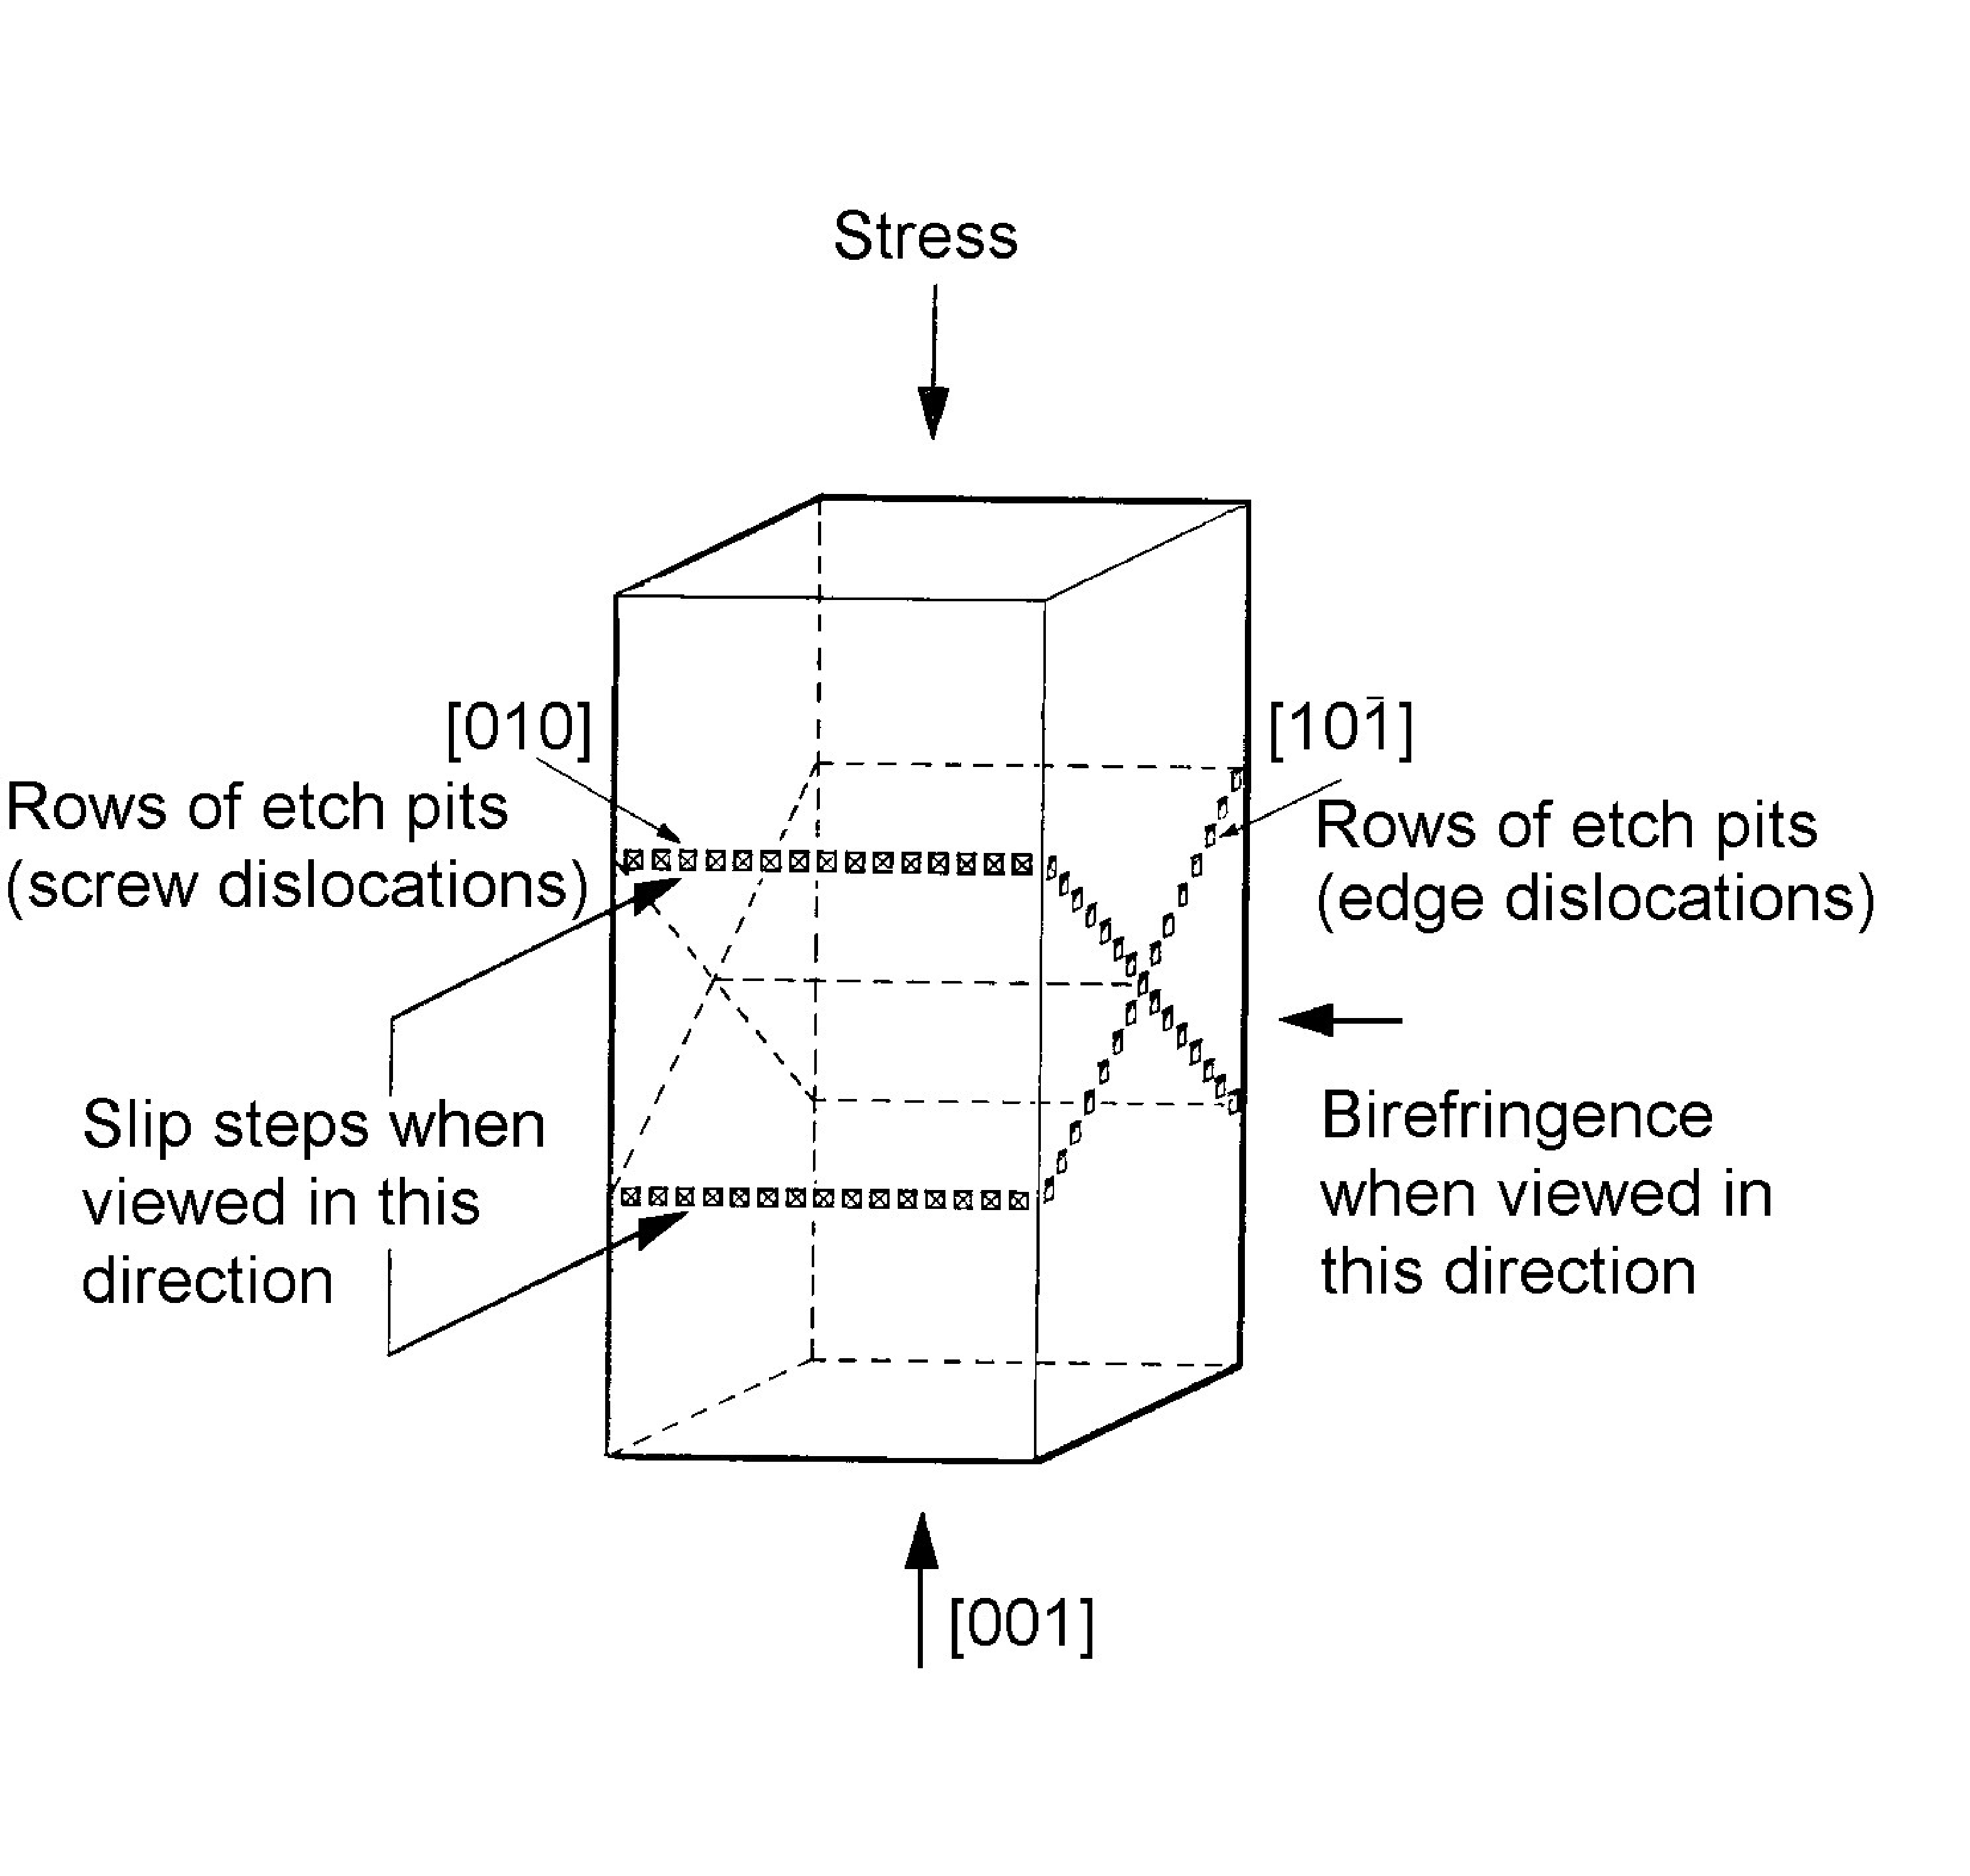
\includegraphics{Dislocations-Fig_19.pdf}

\hypertarget{winkel-zwischen-uxe4tzgruxfcbchen}{%
\subsection{Winkel zwischen
Ätzgrübchen}\label{winkel-zwischen-uxe4tzgruxfcbchen}}

Für den Winkel zwischen den Kristalliten \(\theta\), die in einer
Korngrenze aufeinander treffen, lässt sich geometrisch folgender
Zusammenhang zum Abstand \(d\) zweier Ätzgrübchen und dem Betrag \(b\)
des Burgers-Vektors finden.

\[
\begin{eqnarray}
    \sin(\theta) &=& \frac{b}{d}
\end{eqnarray}
\] Ist die Korngrenze eine Kleinwinkelkorngrenze
(\(\theta < 15^\circ\)), so lässt sich die Kleinwinkelnäherung für den
Sinus nutzen.

\[
\begin{eqnarray}
    \sin(\theta) &\approx& \theta \\
    \Rightarrow \theta &\approx& \frac{b}{d}
\end{eqnarray}
\] Der wahrscheinlichste Burgers-Vektor \(\vec{b}\) für \(\mathrm{LiF}\)
ist wie beschrieben der Vektor \([\frac{1}{2}\,0\,\frac{1}{2}]\) mit
einer Länge von \(b = \frac{a}{\sqrt{2}}\). \[
\begin{eqnarray}
    \theta &\approx& \frac{a}{\sqrt{2} \cdot d} \\
        &=& \frac{0.402\,\mathrm{nm}}{\sqrt{2} d}\\
        &\approx& \frac{0.284\,\mathrm{nm}}{d}
\end{eqnarray}
\]

\hypertarget{durchfuxfchrung}{%
\section{Durchführung}\label{durchfuxfchrung}}

\hypertarget{vorbereitung-der-proben}{%
\subsection{Vorbereitung der Proben}\label{vorbereitung-der-proben}}

Eine Probe \(\mathrm{LiF}\)-Kristall mit äußeren Abmessungen von etwa
\(15 \times 3 \times 3 \,\mathrm{mm^3}\) wird zur Verfügung gestellt. Es
wurde zuvor von einem größeren Kristall durch Spalten abgetrennt und
dann für \(48\) Stunden bei \(650\,^\circ\mathrm C\) getempert und
langsam abgekühlt.

Eine zweite wird zu Beginn des Versuchs von einem größeren Block
abgespalten. Diese wird nicht getempert, allerdings chemisch poliert und
geätzt.

\hypertarget{polieren-und-uxe4tzen}\) aus
Tetrafluoroborsäure \((\mathrm{HBF_4})\), zu \(30\,\mathrm{Vol\%}\) aus
Salpetersäure \((\mathrm{HNO_3})\) und zu \(60\,\mathrm{Vol\%}\) aus
Wasser \((\mathrm{H_2O})\). Das Ätzmittel ist \(50\,\mathrm{ppm}\)
Eisen(III)-Chlorid \((\mathrm{FeCl_3})\) in destiliertem Wasser.

\hypertarget{literatur}{%
\section{Literatur}\label{literatur}}

\begin{enumerate}
\def\labelenumi{\arabic{enumi}.}
\tightlist
\item
  Dislocations in Lithiumfluoride, C. Newey und R. Davidge, editiert von
  A. Bailey, Online verfügbar unter
  \url{https://ph2.uni-koeln.de/fileadmin/Lehre/PraktikumB/Dislocations_in_Lithium_Fluoride.pdf},
  1965
\item
  C. Kittel, Einführung in die Festkörperphysik, München: Oldenbourg
  Verlag, 2005
\item
  S. Hunklinger, Festkörperphysik, München: Oldenbourg Verlag, 2011
\item
  R. Gross und A. Marx, Festkörperphysik, München: Oldenbourg Verlag,
  2012
\item
  Universität zu Köln, ``Anleitung zum Versuch 2.8 Versetzungen in
  LiF'', Online verfügbar unter
  \url{https://ph2.uni-koeln.de/fileadmin/Lehre/PraktikumB/B28-LiF_tutorial_de.pdf},
  Juni 2013
\end{enumerate}

\end{document}
